%% beamer/knitr slides
%% for Statistical Modeling and Data Visualization course @ UMass
%% Nicholas Reich: nick [at] schoolph.umass.edu


\documentclass[table]{beamer}\usepackage[]{graphicx}\usepackage[]{xcolor}
% maxwidth is the original width if it is less than linewidth
% otherwise use linewidth (to make sure the graphics do not exceed the margin)
\makeatletter
\def\maxwidth{ %
  \ifdim\Gin@nat@width>\linewidth
    \linewidth
  \else
    \Gin@nat@width
  \fi
}
\makeatother

\definecolor{fgcolor}{rgb}{0.345, 0.345, 0.345}
\newcommand{\hlnum}[1]{\textcolor[rgb]{0.686,0.059,0.569}{#1}}%
\newcommand{\hlstr}[1]{\textcolor[rgb]{0.192,0.494,0.8}{#1}}%
\newcommand{\hlcom}[1]{\textcolor[rgb]{0.678,0.584,0.686}{\textit{#1}}}%
\newcommand{\hlopt}[1]{\textcolor[rgb]{0,0,0}{#1}}%
\newcommand{\hlstd}[1]{\textcolor[rgb]{0.345,0.345,0.345}{#1}}%
\newcommand{\hlkwa}[1]{\textcolor[rgb]{0.161,0.373,0.58}{\textbf{#1}}}%
\newcommand{\hlkwb}[1]{\textcolor[rgb]{0.69,0.353,0.396}{#1}}%
\newcommand{\hlkwc}[1]{\textcolor[rgb]{0.333,0.667,0.333}{#1}}%
\newcommand{\hlkwd}[1]{\textcolor[rgb]{0.737,0.353,0.396}{\textbf{#1}}}%
\let\hlipl\hlkwb

\usepackage{framed}
\makeatletter
\newenvironment{kframe}{%
 \def\at@end@of@kframe{}%
 \ifinner\ifhmode%
  \def\at@end@of@kframe{\end{minipage}}%
  \begin{minipage}{\columnwidth}%
 \fi\fi%
 \def\FrameCommand##1{\hskip\@totalleftmargin \hskip-\fboxsep
 \colorbox{shadecolor}{##1}\hskip-\fboxsep
     % There is no \\@totalrightmargin, so:
     \hskip-\linewidth \hskip-\@totalleftmargin \hskip\columnwidth}%
 \MakeFramed {\advance\hsize-\width
   \@totalleftmargin\z@ \linewidth\hsize
   \@setminipage}}%
 {\par\unskip\endMakeFramed%
 \at@end@of@kframe}
\makeatother

\definecolor{shadecolor}{rgb}{.97, .97, .97}
\definecolor{messagecolor}{rgb}{0, 0, 0}
\definecolor{warningcolor}{rgb}{1, 0, 1}
\definecolor{errorcolor}{rgb}{1, 0, 0}
\newenvironment{knitrout}{}{} % an empty environment to be redefined in TeX

\usepackage{alltt}


%       ************************************************
%       **        LaTeX preamble to be used with all 
%	**        statsTeachR labs/handouts.
%
%	Author: Nicholas G Reich
%	Last modified: 14 January 2014
%	************************************************

% \documentclass[table]{beamer}

%	Set theme (a nice plain one)
\usetheme{Malmoe}

%	Use named colors, set main color of theme
%		to match Web site color:
\definecolor{MainColor}{RGB}{10, 74, 109}
\colorlet{MainColorMedium}{MainColor!50}
\colorlet{MainColorLight}{MainColor!20}
\usecolortheme[named=MainColor]{structure} 

%	For tables
%[dvipsnames] [table]
\usepackage{xcolor}

%% calling tabu.sty, assuming a particular directory structure
\usepackage{../../slide-includes/tabu}	% Even fancier than tabulary
\usepackage{multirow}

%	Just for the degree symbol
\usepackage{textcomp}

%	Get rid of footline (page, author, etc. on each slide)
\setbeamertemplate{footline}{}
%	Get rid of navigation buttons
\setbeamertemplate{navigation symbols}{}

%	Make footnotes not ugly
\usepackage{hanging}
\setbeamertemplate{footnote}{\raggedright\hangpara{1em}{1}\makebox[1em][l]{\insertfootnotemark}\footnotesize\insertfootnotetext\par}

%	Text style for code snippets inline in text:
\newcommand{\codeInline}[1]{\texttt{#1}}

%	Text style for emphasis stronger than \emph:
%		(Note, this doesn't toggle the way \emph does.
%			(Note, this can be done, didn't seem worth the trouble.))
\newcommand{\strong}[1]{{\bfseries{#1}}}


%        ******	Define title page	**********************
\setbeamertemplate{title page}{
	{\color{MainColor}
	% There must be a better way than this -vspace at
	%	 the top and bottom of the page to reduce the 
	%	 bottom margin, but I can't find one that works.
	\vspace{-6em}

% 	% Go to a lot of trouble to get the title in a
% 	%	nice box, since customizing a beamer block
% 	%	does not entirely work here (I don't know why)
	\newlength{\titleBoxWidth}
	\setlength{\titleBoxWidth}{\textwidth}
	\addtolength{\titleBoxWidth}{-2.0em}
	\setlength{\fboxsep}{1.0em}
	\setlength{\fboxrule}{0pt}
	\fcolorbox{MainColor!25}{MainColor!25}{
		\parbox{\titleBoxWidth}{
			\raggedright
			\LARGE\textbf{\inserttitle}
		}	% end parbox
	}	% end fcolorbox

	\vfill
	\small{Author: \insertauthor}
	\vspace{\baselineskip}

	\small{\Course}

	\small{\Instructor}
	\vspace{\baselineskip}

	%\small{\emph{This material is part of the \strong{statsTeachR} project}}

	\vspace{0.33\baselineskip}\scriptsize{\emph{\LicenseText}}


		\vspace{-15em}

	}	% end color
	\clearpage
}	% end define title page

%	The following variables are assumed by the standard preamble:
%	Global variable containing module name:
\title{Key concepts in data viz and {\tt ggplot}}
%	Global variable containing module shortname:
%		(Currently unused, may be used in future.)
\newcommand{\ModuleShortname}{introRegression}
%	Global variable containing author name:
\author{Nicholas G Reich}
%	Global variable containing text of license terms:
\newcommand{\LicenseText}{Made available under the Creative Commons Attribution-ShareAlike 3.0 Unported License: http://creativecommons.org/licenses/by-sa/3.0/deed.en\textunderscore US }
%	Instructor: optional, can leave blank.
%		Recommended format: {Instructor: Jane Doe}
\newcommand{\Instructor}{}
%	Course: optional, can leave blank.
%		Recommended format: {Course: Biostatistics 101}
\newcommand{\Course}{}


\input{../../slide-includes/shortcuts}

\hypersetup{colorlinks,linkcolor=,urlcolor=MainColor}


%	******	Document body begins here	**********************
\IfFileExists{upquote.sty}{\usepackage{upquote}}{}
\begin{document}

%	Title page
\begin{frame}[plain]
	\titlepage
\end{frame}

%	******	Everything through the above line must be placed at
%		the top of any TeX file using the statsTeachR standard
%		beamer preamble.


%%%%%%%%%%%%%%%%%%%%%%%%%%%%%%%%%%%%%%%%%%

\begin{frame}

\centering
\Huge Types of data graphics


\end{frame}

%%%%%%%%%%%%%%%%%%%%%%%%%%%%%%%%%%%%%%%%%%

\begin{frame}[fragile]{Using graphics to explore data}

\begin{itemize}
    \item The most valuable graphics are often the simple ones you make for yourself.
    \item Exploratory graphics can introduce you to a dataset.
    \item Key goal: understand the variation.
    \item What do you want to know about these data?
\end{itemize}


\begin{knitrout}
\definecolor{shadecolor}{rgb}{0.969, 0.969, 0.969}\color{fgcolor}\begin{kframe}
\begin{alltt}
\hlkwd{data}\hlstd{(airquality)}
\hlkwd{head}\hlstd{(airquality)}
\end{alltt}
\begin{verbatim}
##   Ozone Solar.R Wind Temp Month Day
## 1    41     190  7.4   67     5   1
## 2    36     118  8.0   72     5   2
## 3    12     149 12.6   74     5   3
## 4    18     313 11.5   62     5   4
## 5    NA      NA 14.3   56     5   5
## 6    28      NA 14.9   66     5   6
\end{verbatim}
\end{kframe}
\end{knitrout}

\end{frame}

%%%%%%%%%%%%%%%%%%%%%%%%%%%%%%%%%%%%%%%%%%

\begin{frame}[fragile]{Exploratory summaries: airquality data}

Understanding what the rows and columns are

\scriptsize
\begin{knitrout}
\definecolor{shadecolor}{rgb}{0.969, 0.969, 0.969}\color{fgcolor}\begin{kframe}
\begin{alltt}
\hlkwd{nrow}\hlstd{(airquality)}
\end{alltt}
\begin{verbatim}
## [1] 153
\end{verbatim}
\begin{alltt}
\hlkwd{str}\hlstd{(airquality)}
\end{alltt}
\begin{verbatim}
## 'data.frame':	153 obs. of  6 variables:
##  $ Ozone  : int  41 36 12 18 NA 28 23 19 8 NA ...
##  $ Solar.R: int  190 118 149 313 NA NA 299 99 19 194 ...
##  $ Wind   : num  7.4 8 12.6 11.5 14.3 14.9 8.6 13.8 20.1 8.6 ...
##  $ Temp   : int  67 72 74 62 56 66 65 59 61 69 ...
##  $ Month  : int  5 5 5 5 5 5 5 5 5 5 ...
##  $ Day    : int  1 2 3 4 5 6 7 8 9 10 ...
\end{verbatim}
\end{kframe}
\end{knitrout}

\end{frame}

%%%%%%%%%%%%%%%%%%%%%%%%%%%%%%%%%%%%%%%%%%

\begin{frame}[fragile]{Exploratory summaries: airquality data}

Tabulating different values of the data using

\scriptsize
\begin{knitrout}
\definecolor{shadecolor}{rgb}{0.969, 0.969, 0.969}\color{fgcolor}\begin{kframe}
\begin{alltt}
\hlkwd{stem}\hlstd{(airquality}\hlopt{$}\hlstd{Ozone)}
\end{alltt}
\begin{verbatim}
## 
##   The decimal point is 1 digit(s) to the right of the |
## 
##    0 | 1467778999
##    1 | 01112233334444666688889
##    2 | 0000111123333334478889
##    3 | 001222455667799
##    4 | 01444556789
##    5 | 0299
##    6 | 134456
##    7 | 13367889
##    8 | 024559
##    9 | 1677
##   10 | 8
##   11 | 058
##   12 | 2
##   13 | 5
##   14 | 
##   15 | 
##   16 | 8
\end{verbatim}
\end{kframe}
\end{knitrout}

\end{frame}

%%%%%%%%%%%%%%%%%%%%%%%%%%%%%%%%%%%%%%%%%%

\begin{frame}[fragile]{Exploratory summaries: airquality data}

Tabulating different values of the data

\scriptsize
\begin{knitrout}
\definecolor{shadecolor}{rgb}{0.969, 0.969, 0.969}\color{fgcolor}\begin{kframe}
\begin{alltt}
\hlkwd{table}\hlstd{(airquality}\hlopt{$}\hlstd{Month)}
\end{alltt}
\begin{verbatim}
## 
##  5  6  7  8  9 
## 31 30 31 31 30
\end{verbatim}
\begin{alltt}
\hlkwd{with}\hlstd{(airquality,} \hlkwd{table}\hlstd{(Month, Day))}
\end{alltt}
\begin{verbatim}
##      Day
## Month 1 2 3 4 5 6 7 8 9 10 11 12 13 14 15 16 17 18 19 20 21 22 23 24 25 26 27
##     5 1 1 1 1 1 1 1 1 1  1  1  1  1  1  1  1  1  1  1  1  1  1  1  1  1  1  1
##     6 1 1 1 1 1 1 1 1 1  1  1  1  1  1  1  1  1  1  1  1  1  1  1  1  1  1  1
##     7 1 1 1 1 1 1 1 1 1  1  1  1  1  1  1  1  1  1  1  1  1  1  1  1  1  1  1
##     8 1 1 1 1 1 1 1 1 1  1  1  1  1  1  1  1  1  1  1  1  1  1  1  1  1  1  1
##     9 1 1 1 1 1 1 1 1 1  1  1  1  1  1  1  1  1  1  1  1  1  1  1  1  1  1  1
##      Day
## Month 28 29 30 31
##     5  1  1  1  1
##     6  1  1  1  0
##     7  1  1  1  1
##     8  1  1  1  1
##     9  1  1  1  0
\end{verbatim}
\end{kframe}
\end{knitrout}

\end{frame}

%%%%%%%%%%%%%%%%%%%%%%%%%%%%%%%%%%%%%%%%%%

\begin{frame}[fragile]{Univariate graphics: airquality data}

{\bf Univariate graphics} show you the distribution of or the variation in the observations of a single variable.

\begin{knitrout}
\definecolor{shadecolor}{rgb}{0.969, 0.969, 0.969}\color{fgcolor}
\includegraphics[width=\maxwidth]{figure/unnamed-chunk-5-1} 
\end{knitrout}

\end{frame}


%%%%%%%%%%%%%%%%%%%%%%%%%%%%%%%%%%%%%%%%%%

\begin{frame}[fragile]{Bivariate graphics: airquality data}

{\bf Bivariate graphics} show you the relationship between two variables in your dataset.

\begin{knitrout}
\definecolor{shadecolor}{rgb}{0.969, 0.969, 0.969}\color{fgcolor}
\includegraphics[width=\maxwidth]{figure/unnamed-chunk-6-1} 
\end{knitrout}

\end{frame}

%%%%%%%%%%%%%%%%%%%%%%%%%%%%%%%%%%%%%%%%%%

\begin{frame}[fragile]{Bivariate graphics: pairs plots!}

Pairs plots are nice, but can take some time to render (especially for big datasets).
\begin{knitrout}
\definecolor{shadecolor}{rgb}{0.969, 0.969, 0.969}\color{fgcolor}\begin{kframe}
\begin{alltt}
\hlstd{GGally}\hlopt{::}\hlkwd{ggpairs}\hlstd{(airquality)}
\end{alltt}
\end{kframe}
\includegraphics[width=\maxwidth]{figure/unnamed-chunk-7-1} 
\end{knitrout}

\end{frame}


%%%%%%%%%%%%%%%%%%%%%%%%%%%%%%%%%%%%%%%%%%

\begin{frame}[fragile]{Multivariate graphics}

{\bf Multivariate graphics} show you the relationship between multiple variables in your dataset. Rather than using some fancy "3D" plot, it is often better to use other features like color or shapes or facets to show a third or fourth variable.

\begin{knitrout}
\definecolor{shadecolor}{rgb}{0.969, 0.969, 0.969}\color{fgcolor}
\includegraphics[width=\maxwidth]{figure/unnamed-chunk-8-1} 
\end{knitrout}

\end{frame}


%%%%%%%%%%%%%%%%%%%%%%%%%%%%%%%%%%%%%%%%%%

\begin{frame}

\centering
\Huge Using {\tt ggplot}


\end{frame}

%%%%%%%%%%%%%%%%%%%%%%%%%%%%%%%%%%%%%%%%%%

\begin{frame}{Choices for R graphics}

You have three central choices for making graphics in R:

\begin{itemize}
    \item ``Base R graphics''
    \item {\tt ggplot2}
    \item lattice
\end{itemize}

\vspace{2em}

I use {\tt ggplot} because:
\begin{enumerate}
    \item it is integrated with the {\tt tidyverse}
    \item it is actively developed/maintained
    \item there are a ton of extensions (see more later)
\end{enumerate}


\end{frame}


%%%%%%%%%%%%%%%%%%%%%%%%%%%%%%%%%%%%%%%%%%

\begin{frame}[fragile]{Understanding the ``grammar'' of ggplot2}

The grammar ...

\begin{itemize}
    \item layers (a `geom', a `stat', an `annotation')
    \item aesthetics (`aes`)
    \item scales
    \item facets
    \item data
    \item ... and more here: \href{http://ggplot2.tidyverse.org/reference/}{http://ggplot2.tidyverse.org/reference/}
\end{itemize}

\end{frame}

%%%%%%%%%%%%%%%%%%%%%%%%%%%%%%%%%%%%%%%%%%

\begin{frame}[fragile]{What is a layer?}


\begin{block}{Layers define the basic structure of the elements on the plot}
\begin{itemize}
    \item \href{https://ggplot2.tidyverse.org/reference/#section-geoms}{Geoms}: point, line, tile, boxplot, ribbon, ...
    \item \href{https://ggplot2.tidyverse.org/reference/#section-stats}{Stats}: histogram, smooth, density, ...
    \item \href{https://ggplot2.tidyverse.org/reference/#section-annotations}{Annotation}: hline, vline, text, ...
\end{itemize}

For more info check out the documentation: \href{http://ggplot2.tidyverse.org/reference/}{http://ggplot2.tidyverse.org/reference/}.

\end{block}

\end{frame}

%%%%%%%%%%%%%%%%%%%%%%%%%%%%%%%%%%%%%%%%%%

\begin{frame}[fragile]{What are ``aesthetics''?}

Aesthetics define a mapping between {\bf tidy data} and the information required to create a specific graphic\footnote{Figure credits: Hadley Wickham}

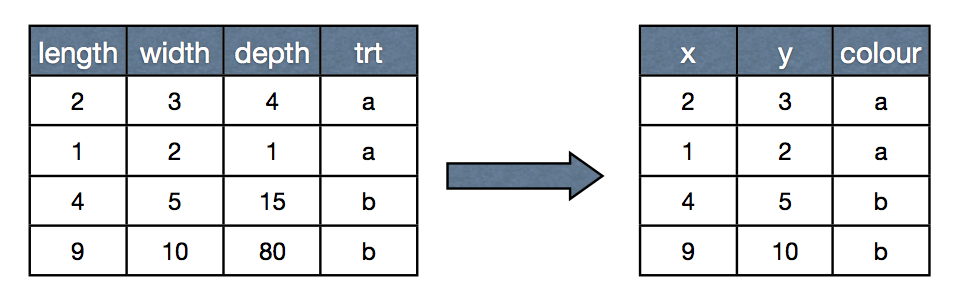
\includegraphics[width=\textwidth]{figure-static/aes.png}

\end{frame}


%%%%%%%%%%%%%%%%%%%%%%%%%%%%%%%%%%%%%%%%%%

\begin{frame}[fragile]{\tt{geom\_point}}


Each geom has a different set of aesthetics.

What information do we need to draw a scatterplot? \\
Or, asked another way, what aesthetics do we need for {\tt geom\_point}?

\uncover<2>{
\begin{itemize}
    \item x (required)
    \item y (required)
    \item alpha
    \item color
    \item fill
    \item shape
    \item size
\end{itemize}
}
\end{frame}


%%%%%%%%%%%%%%%%%%%%%%%%%%%%%%%%%%%%%%%%%%

\begin{frame}[fragile]{\tt{geom\_point}}

\scriptsize
\begin{knitrout}
\definecolor{shadecolor}{rgb}{0.969, 0.969, 0.969}\color{fgcolor}\begin{kframe}
\begin{alltt}
\hlkwd{library}\hlstd{(ggplot2)}
\hlkwd{theme_set}\hlstd{(}\hlkwd{theme_bw}\hlstd{())}
\hlkwd{ggplot}\hlstd{(airquality)} \hlopt{+}
  \hlkwd{geom_point}\hlstd{(}\hlkwd{aes}\hlstd{(}\hlkwc{x}\hlstd{=Temp,} \hlkwc{y}\hlstd{=Ozone,} \hlkwc{color}\hlstd{=}\hlkwd{factor}\hlstd{(Month),} \hlkwc{size}\hlstd{=Wind))}
\end{alltt}
\end{kframe}
\includegraphics[width=\maxwidth]{figure/unnamed-chunk-9-1} 
\end{knitrout}


\end{frame}
%%%%%%%%%%%%%%%%%%%%%%%%%%%%%%%%%%%%%%%%%%

\begin{frame}[fragile]{\tt{geom\_line}}

What information do we need to draw a line of connected points? \\
Or, asked another way, what aesthetics do we need for {\tt geom\_line}?

\uncover<2>{
\begin{itemize}
    \item x (required)
    \item y (required)
    \item alpha
    \item color
    \item linetype
    \item size
\end{itemize}
}
\end{frame}


%%%%%%%%%%%%%%%%%%%%%%%%%%%%%%%%%%%%%%%%%%

\begin{frame}[fragile]{\tt{geom\_line}}

\scriptsize
\begin{knitrout}
\definecolor{shadecolor}{rgb}{0.969, 0.969, 0.969}\color{fgcolor}\begin{kframe}
\begin{alltt}
\hlstd{airquality}\hlopt{$}\hlstd{Date} \hlkwb{<-} \hlstd{lubridate}\hlopt{::}\hlkwd{ymd}\hlstd{(}\hlkwd{paste}\hlstd{(}\hlnum{1973}\hlstd{, airquality}\hlopt{$}\hlstd{Month, airquality}\hlopt{$}\hlstd{Day))}
\hlkwd{ggplot}\hlstd{(airquality,} \hlkwd{aes}\hlstd{(}\hlkwc{x}\hlstd{=Date,} \hlkwc{y}\hlstd{=Temp))} \hlopt{+}
  \hlkwd{geom_line}\hlstd{()} \hlopt{+} \hlkwd{geom_point}\hlstd{(}\hlkwd{aes}\hlstd{(}\hlkwc{color}\hlstd{=Ozone))} \hlopt{+}
  \hlkwd{scale_color_gradient}\hlstd{(}\hlkwc{low}\hlstd{=}\hlstr{"green"}\hlstd{,} \hlkwc{high}\hlstd{=}\hlstr{"red"}\hlstd{)}
\end{alltt}
\end{kframe}
\includegraphics[width=\maxwidth]{figure/unnamed-chunk-10-1} 
\end{knitrout}


\end{frame}


%%%%%%%%%%%%%%%%%%%%%%%%%%%%%%%%%%%%%%%%%%


\begin{frame}[fragile]{}

\centering
\Large
{\tt ggplot} extensions that I used in \href{https://www.medrxiv.org/content/10.1101/2021.02.03.21250974v1}{a recent paper}

\end{frame}


\begin{frame}[fragile]{{\tt gridExtra} or {\tt cowplot} for multi-plot alignment}

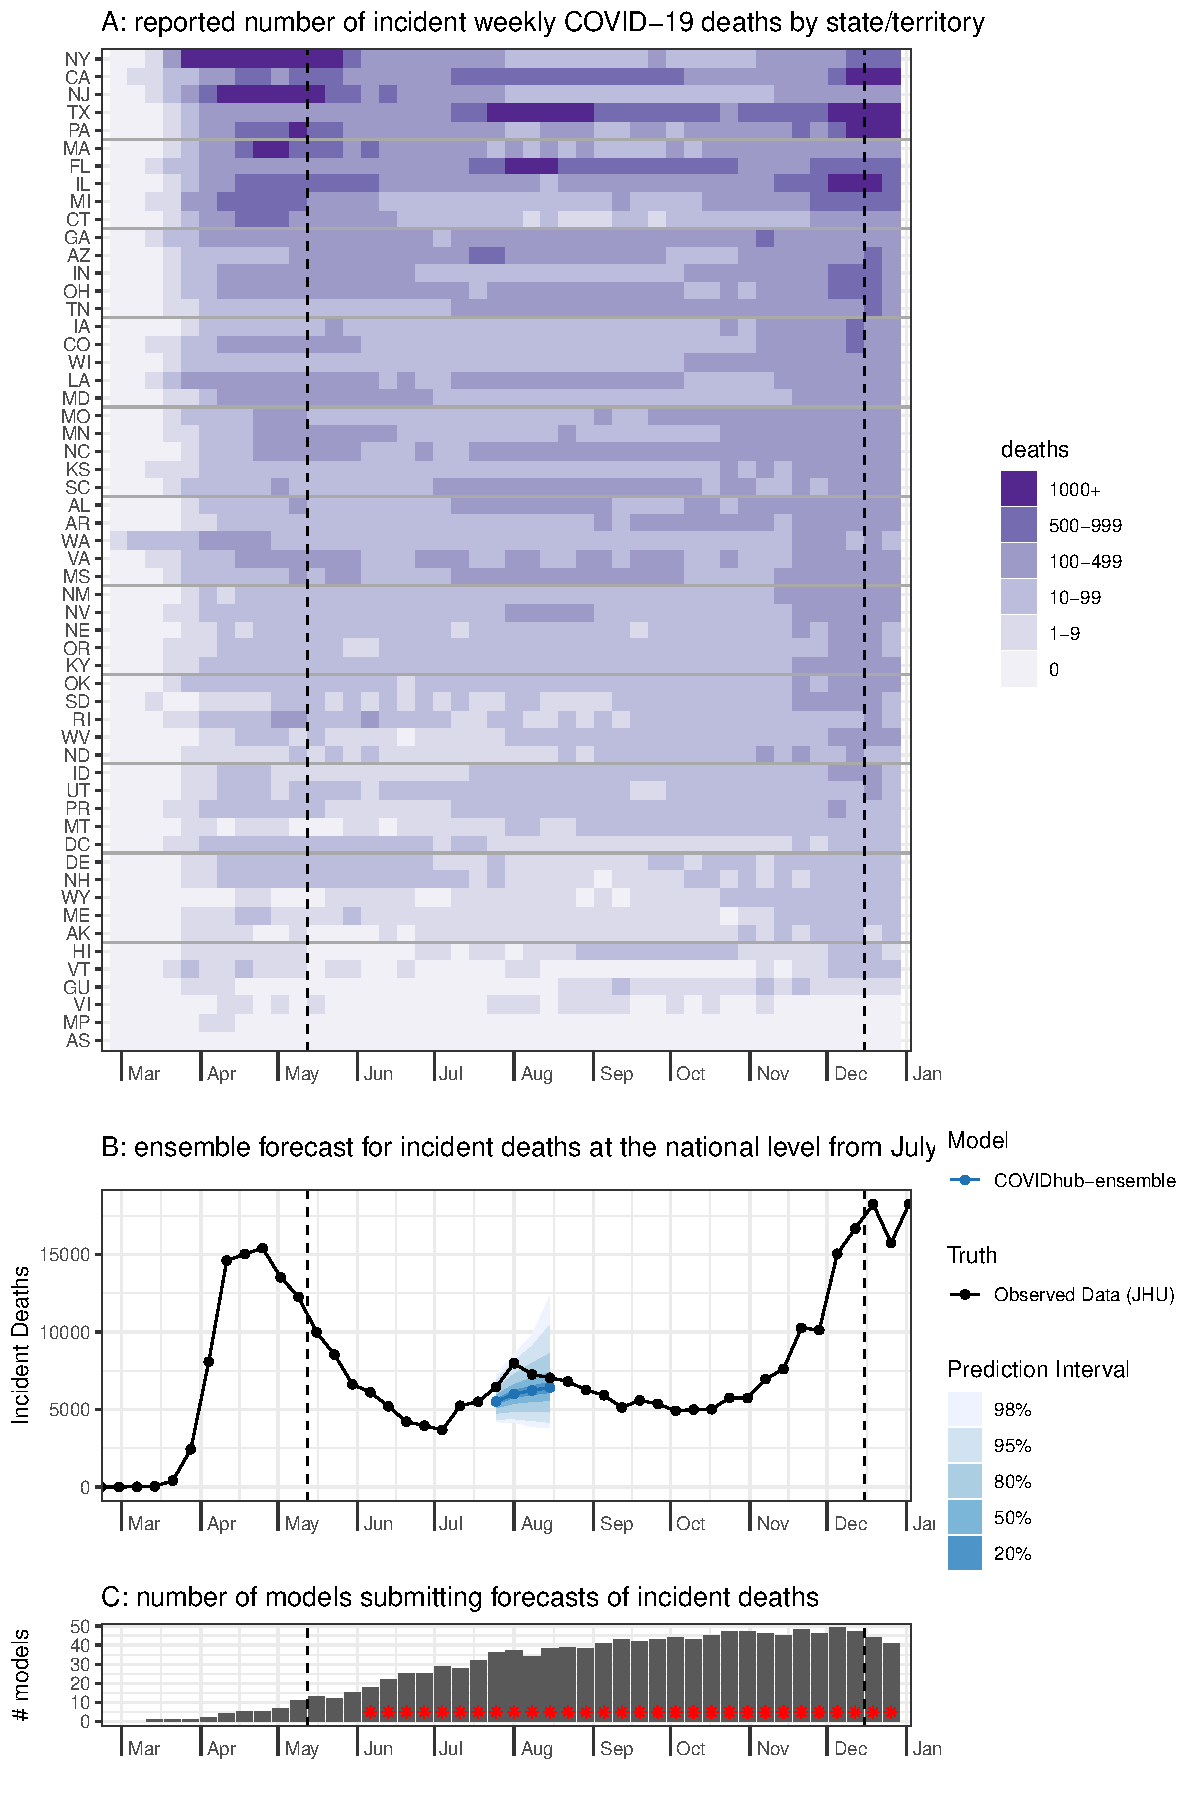
\includegraphics[width=.5\textwidth]{figure-static/data-and-forecast}

\end{frame}


\begin{frame}[fragile]{\href{https://wilkelab.org/ggridges/}{{\tt ggrides}} for ridgeplots}

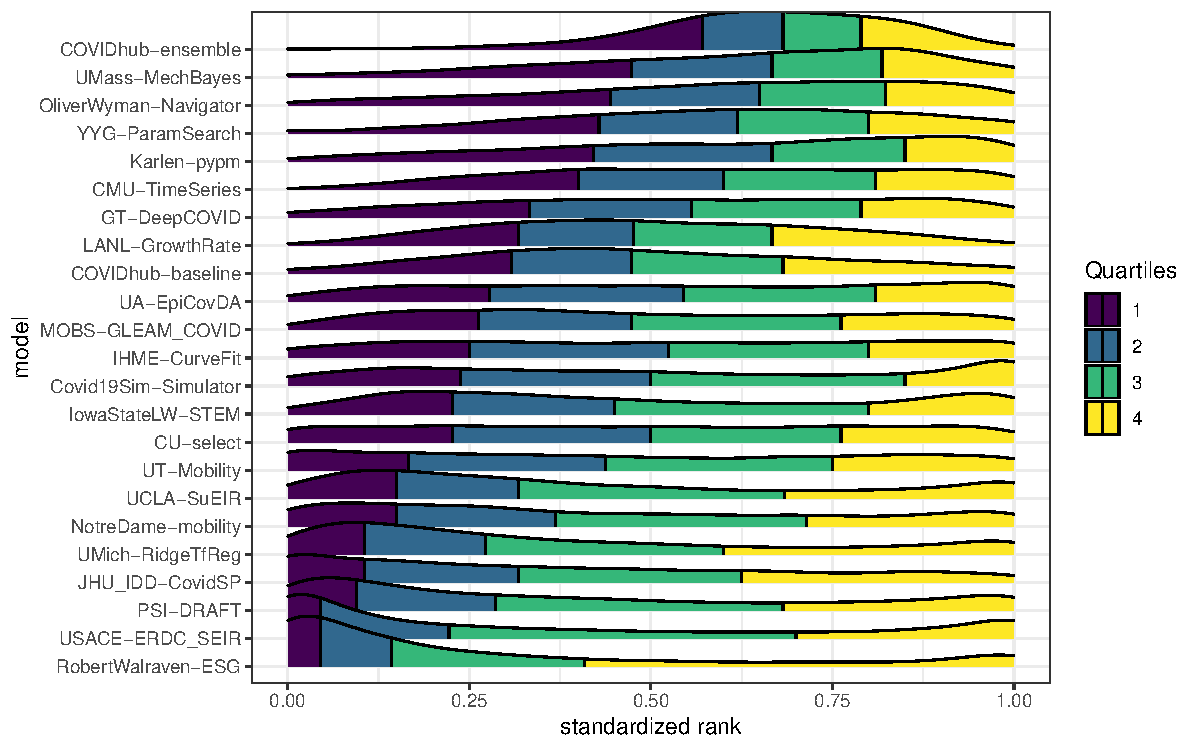
\includegraphics[width=\textwidth]{figure-static/fig-model-ranks}

\end{frame}


\begin{frame}[fragile]{{\tt RColorBrewer} and {\tt viridis} for colors}

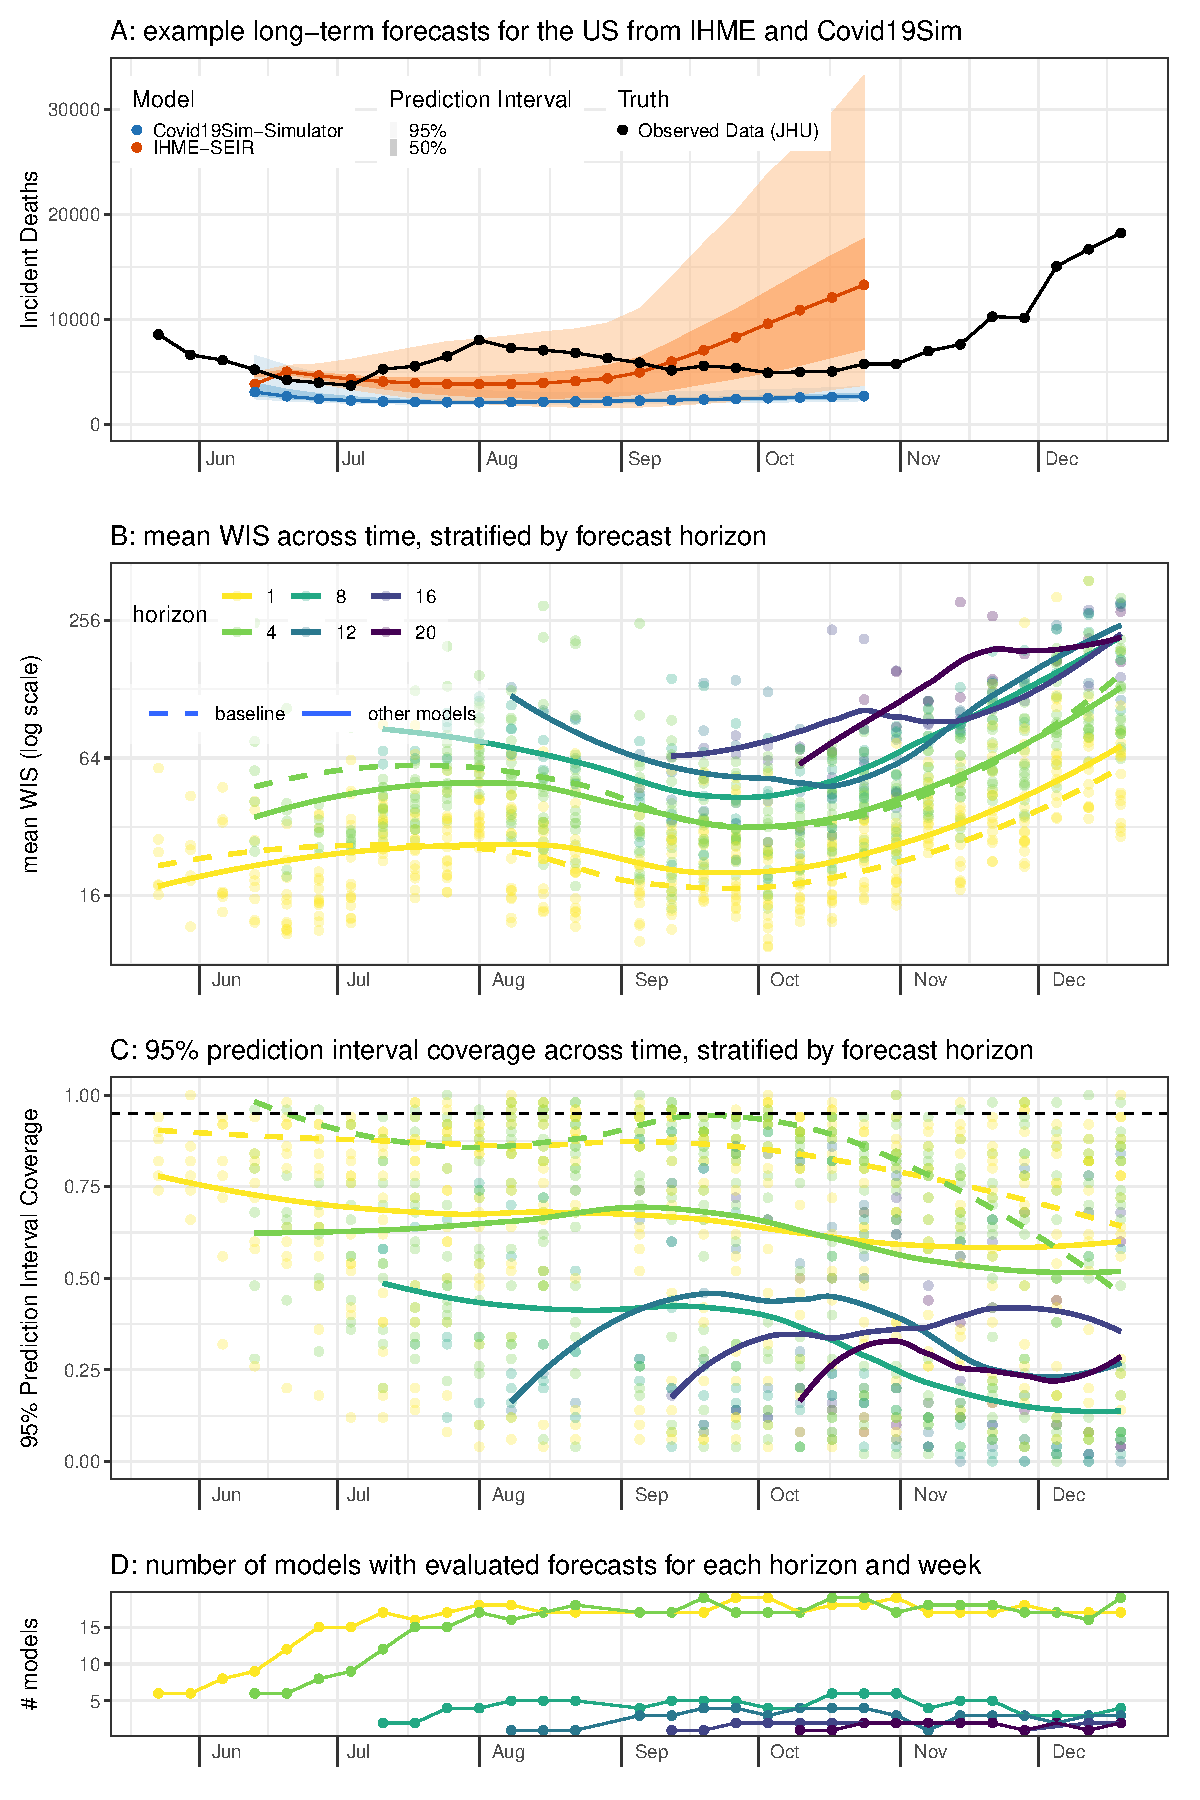
\includegraphics[width=.5\textwidth]{figure-static/fig-by-horizon-week}

\end{frame}


%%%%%%%%%%%%%%%%%%%%%%%%%%%%%%%%%%%%%%%%%%


\begin{frame}[fragile]{Note-catcher}


A figure from \href{http://www.pnas.org/content/112/16/4999.full.pdf}{``Cities, traffic, and CO2: A multidecadal assessment of trends, drivers, and scaling relationships'', Gately et al, PNAS, 2015.} Original paper on Moodle.

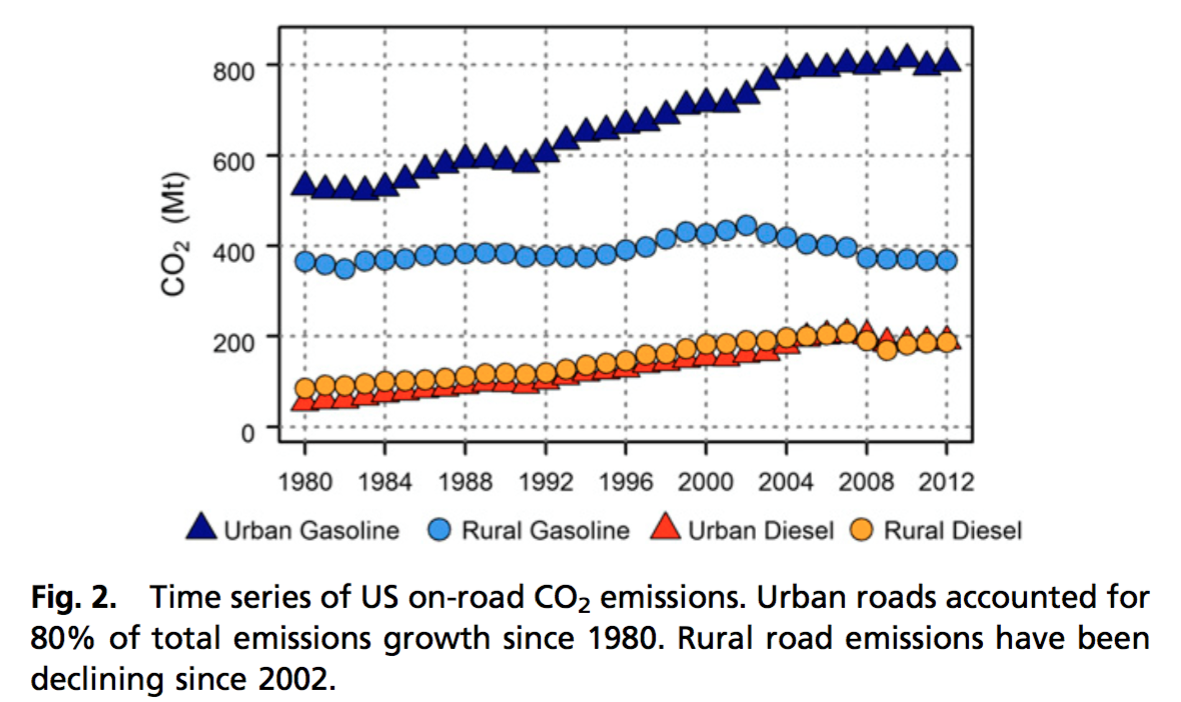
\includegraphics[width=\textwidth]{figure-static/pollution.png}

\end{frame}


%%%%%%%%%%%%%%%%%%%%%%%%%%%%%%%%%%%%%%%%%%


\begin{frame}[fragile]{Note-catcher}

We have made the data from the CO2 emissions figure available on Canvas. As a group, you will be asked to complete the following tasks:

\begin{enumerate}
    \item Recreate the figure as close as possible to the original.
    \item Improve the figure. Make some changes that you think make the figure more clear.
    \item Post your final figures on the Note-catcher document.
\end{enumerate}

The class will vote on which figure is (1) closest to the original and (2) the best improvement. Extra credit on a future homework assignment will be awarded to all members at the table(s) that win the votes.

\begin{block}{NOTE}
Everyone should be doing some coding here, and having a version of the graphic working on their laptop! Make sure it's not just 1-2 people typing the code and having it work for them.
\end{block}

\end{frame}





\end{document}
